\documentclass[tikz,border=7pt]{standalone}
\usetikzlibrary{angles,quotes}
\begin{document}
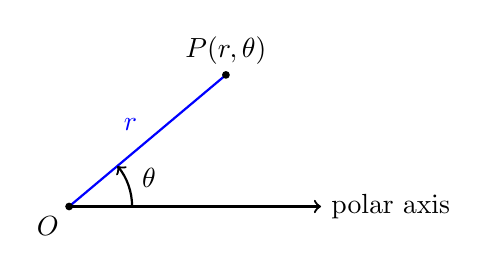
\begin{tikzpicture}[line width=.8pt]
\coordinate (O) at (0,0); \coordinate (X) at (3.2,0); \coordinate (P) at (40:2.6);
\draw[->] (O)--(X) node[right] {polar axis}; \draw[blue,thick] (O)--(P) node[midway,above left] {$r$};
\pic[draw,->,"$\theta$",angle radius=.8cm,angle eccentricity=1.35] {angle=X--O--P};
\fill (O) circle (1.4pt) node[below left] {$O$}; \fill (P) circle (1.4pt) node[above] {$P(r,\theta)$};
\end{tikzpicture}
\end{document}
